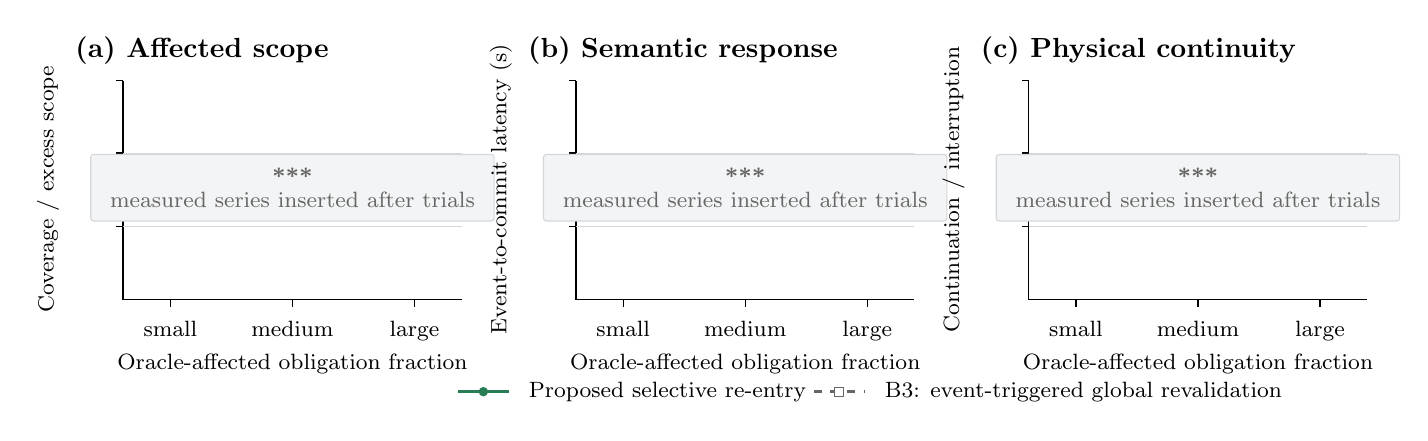
\begin{tikzpicture}[x=1cm,y=1cm,font=\rmfamily\fontsize{8.2}{9.0}\selectfont]
  \definecolor{expours}{HTML}{287D55}
  \definecolor{expbase}{HTML}{666666}
  \definecolor{expgrid}{HTML}{D4D7DA}
  \definecolor{expnote}{HTML}{F3F4F5}

  % Three final-result panels. The empty axes deliberately encode no data.
  \foreach \x/\panel/\title/\ylabel in {
    0.0/{(a)}/{Affected scope}/{Coverage / excess scope},
    5.75/{(b)}/{Semantic response}/{Event-to-commit latency (s)},
    11.50/{(c)}/{Physical continuity}/{Continuation / interruption}
  }{
    \begin{scope}[shift={(\x,0)}]
      \draw[black,line width=0.6pt] (0.75,0.62) -- (5.05,0.62);
      \draw[black,line width=0.6pt] (0.75,0.62) -- (0.75,3.40);
      \draw[expgrid,line width=0.35pt] (0.75,1.55) -- (5.05,1.55);
      \draw[expgrid,line width=0.35pt] (0.75,2.48) -- (5.05,2.48);
      \foreach \tx/\lab in {1.35/{small},2.90/{medium},4.45/{large}}{
        \draw[black,line width=0.45pt] (\tx,0.62) -- (\tx,0.53);
        \node[anchor=north] at (\tx,0.47) {\lab};
      }
      \foreach \ty in {1.55,2.48,3.40}{
        \draw[black,line width=0.45pt] (0.75,\ty) -- (0.66,\ty);
      }
      \node[font=\bfseries,anchor=west] at (0.02,3.78) {\panel\ \title};
      \node[anchor=north] at (2.90,0.05) {Oracle-affected obligation fraction};
      \node[rotate=90,anchor=south] at (0.06,2.02) {\ylabel};
      \node[draw=expgrid,fill=expnote,rounded corners=1pt,align=center,
            text=expbase,inner xsep=7pt,inner ysep=5pt] at (2.90,2.04)
            {\bfseries ***\\[-1pt]\normalfont measured series inserted after trials};
    \end{scope}
  }

  \draw[expours,line width=1.05pt] (5.00,-0.55) -- (5.65,-0.55);
  \fill[expours] (5.325,-0.55) circle (1.7pt);
  \node[anchor=west] at (5.78,-0.55) {Proposed selective re-entry};
  \draw[expbase,dashed,line width=0.95pt] (9.52,-0.55) -- (10.17,-0.55);
  \node[draw=expbase,fill=white,minimum size=3.2pt,inner sep=0pt]
        at (9.845,-0.55) {};
  \node[anchor=west] at (10.30,-0.55) {B3: event-triggered global revalidation};
  \path[use as bounding box] (-0.05,-0.82) rectangle (16.65,3.98);
\end{tikzpicture}
